\section*{Appendix A: GCFT Field Visualizations}
\addcontentsline{toc}{section}{Appendix A: GCFT Field Visualizations}

This appendix presents selected visualizations of the coherence field $\Xi$, illustrating core GCFT principles: phase curvature, coherence locking, rebound modes, and mass-generating field structures. Each panel depicts a physically consistent configuration, highlighting the emergence of particle properties from field topology.

\vspace{1em}

\renewcommand{\thefigure}{A\arabic{figure}}
\setcounter{figure}{0}

\noindent
\begin{minipage}{0.48\textwidth}
\centering
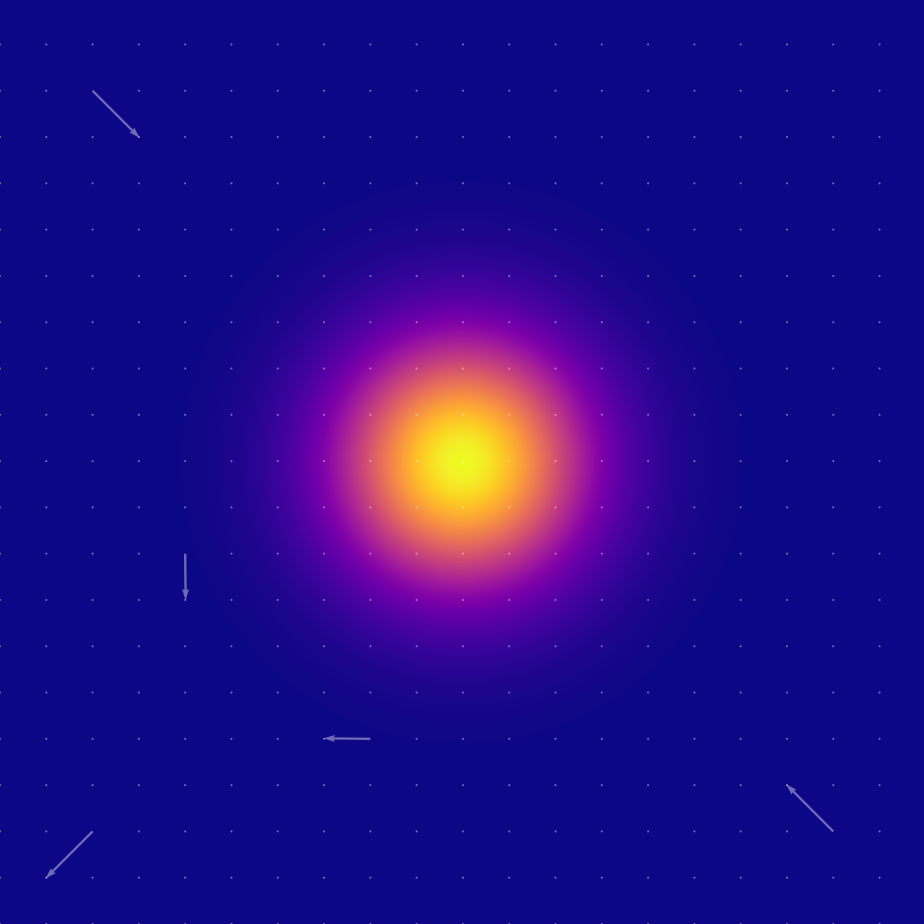
\includegraphics[width=\linewidth]{figures/xi_core_modulus_vector_overlay.png}
\captionof{figure}{$\Xi$--Core Resonance: Localized compression models massive field nodes.}
\end{minipage}
\hfill
\begin{minipage}{0.48\textwidth}
\centering
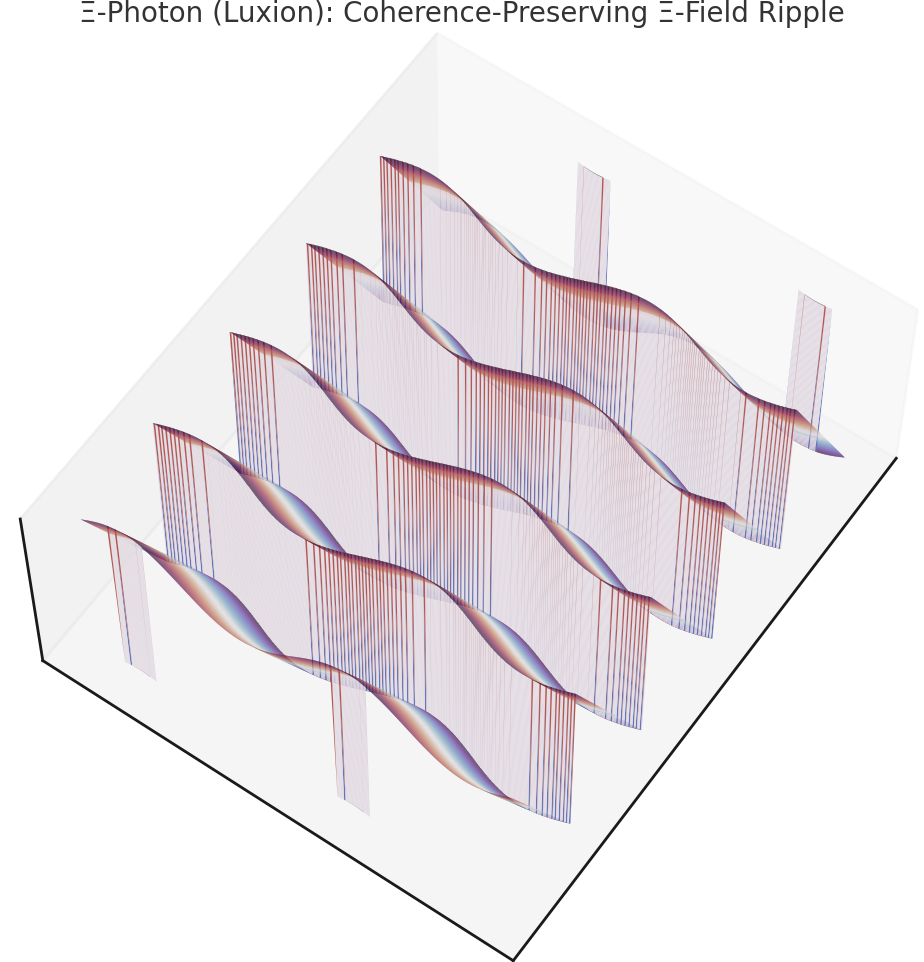
\includegraphics[width=\linewidth]{figures/xi_photon_phase_surface.png}
\captionof{figure}{$\Xi$--Luxion Phase: Pure phase wavefront, illustrating a GCFT photon.}
\end{minipage}

\vspace{1.2em}

\noindent
\begin{minipage}{0.48\textwidth}
\centering
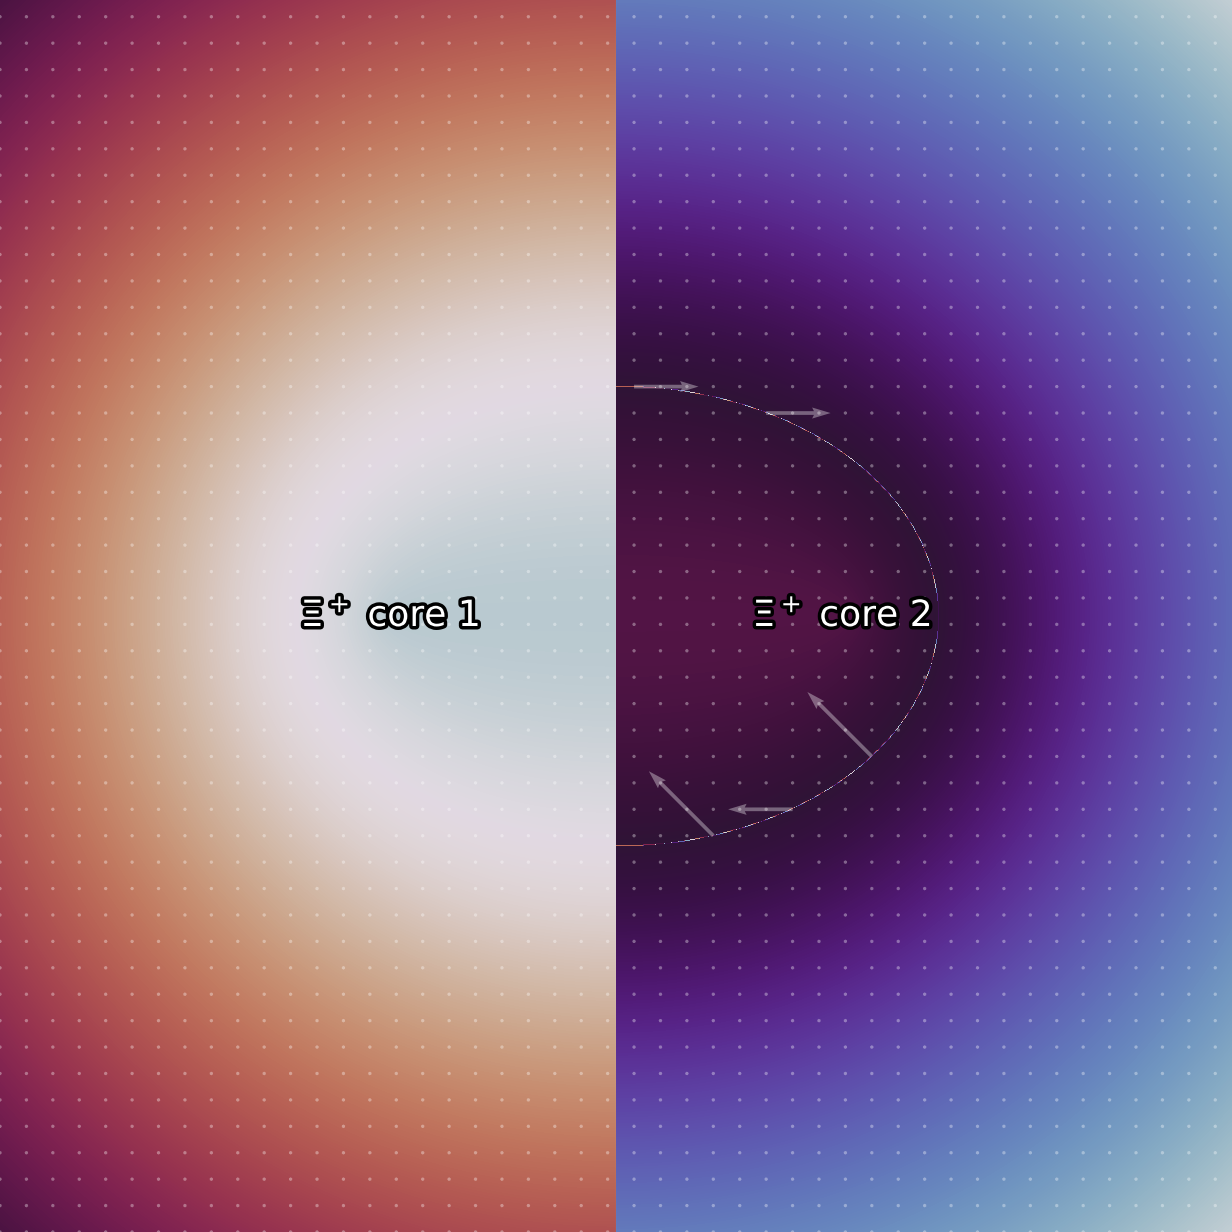
\includegraphics[width=\linewidth]{figures/pion_phase_final.png}
\captionof{figure}{$\Xi$--Pion Rebound: Symmetric lobes, transient phase-coherent loop.}
\end{minipage}
\hfill
\begin{minipage}{0.48\textwidth}
\centering
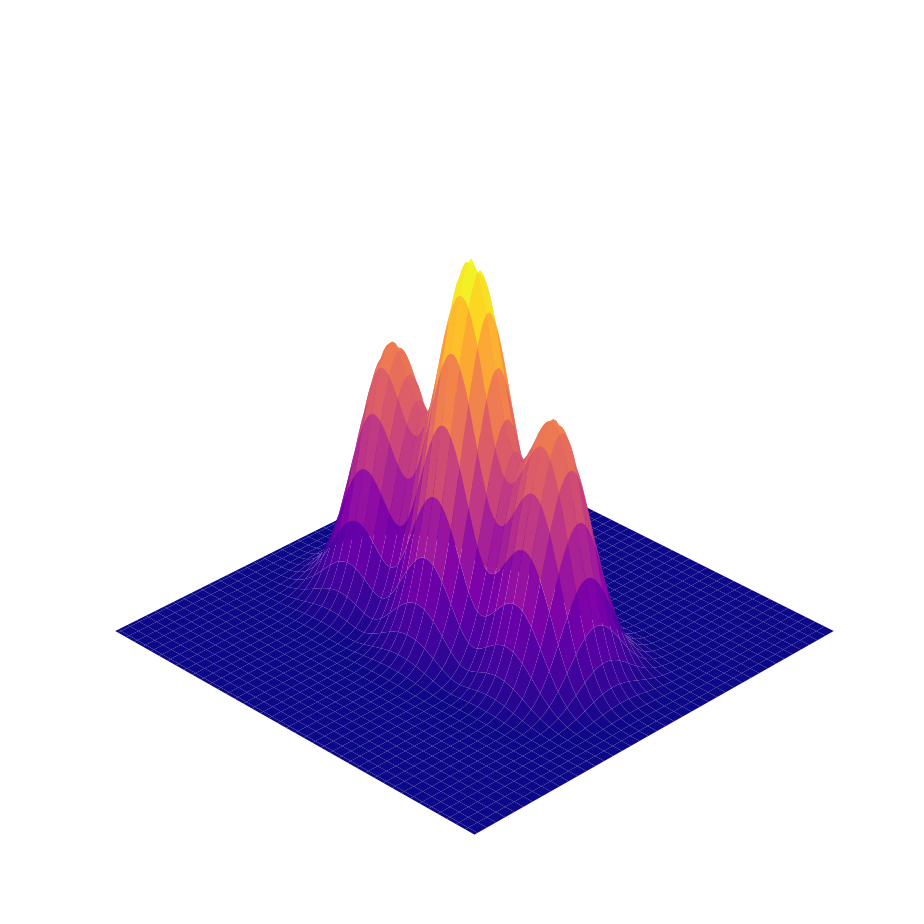
\includegraphics[width=\linewidth]{figures/xi_time_crystal_3d_surface.png}
\captionof{figure}{$\Xi$--Time Crystal: Stable resonance with temporal symmetry breaking.}
\end{minipage}

\vspace{1.2em}

\noindent
\begin{minipage}{0.48\textwidth}
\centering
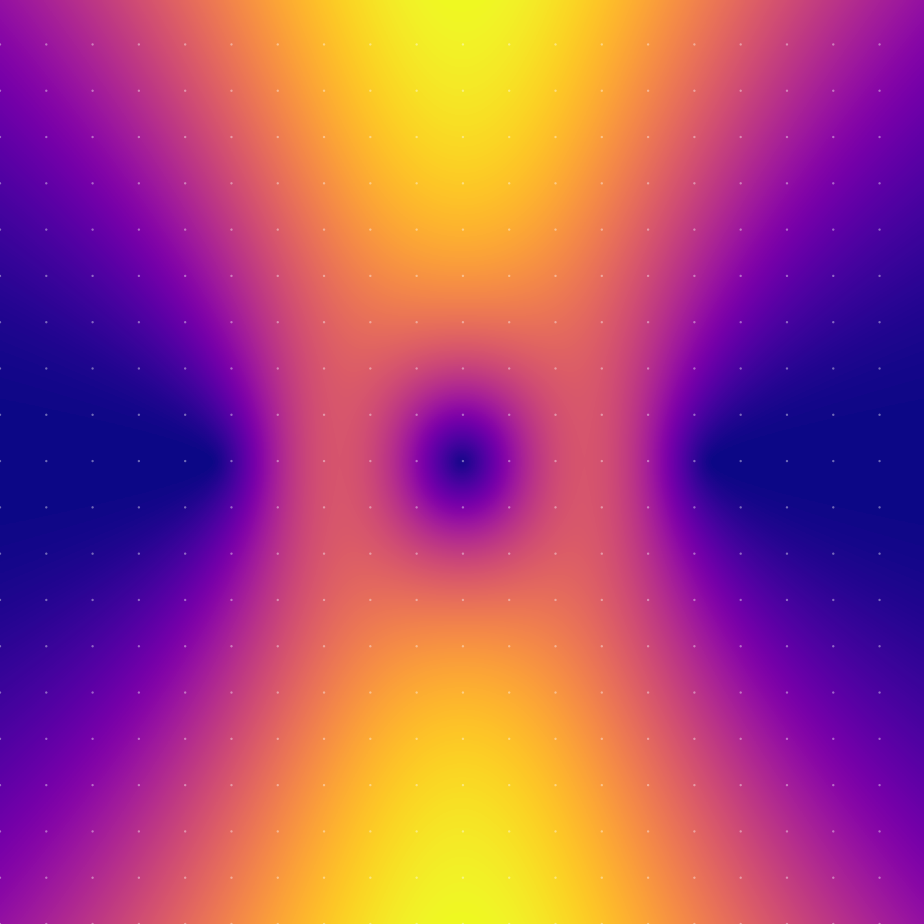
\includegraphics[width=\linewidth]{figures/helium_modulus_vector_overlay.png}
\captionof{figure}{$\Xi$--Helium Lock: Two phase-locked $\Xi$-electrons and a core.}
\end{minipage}
\hfill
\begin{minipage}{0.48\textwidth}
\centering
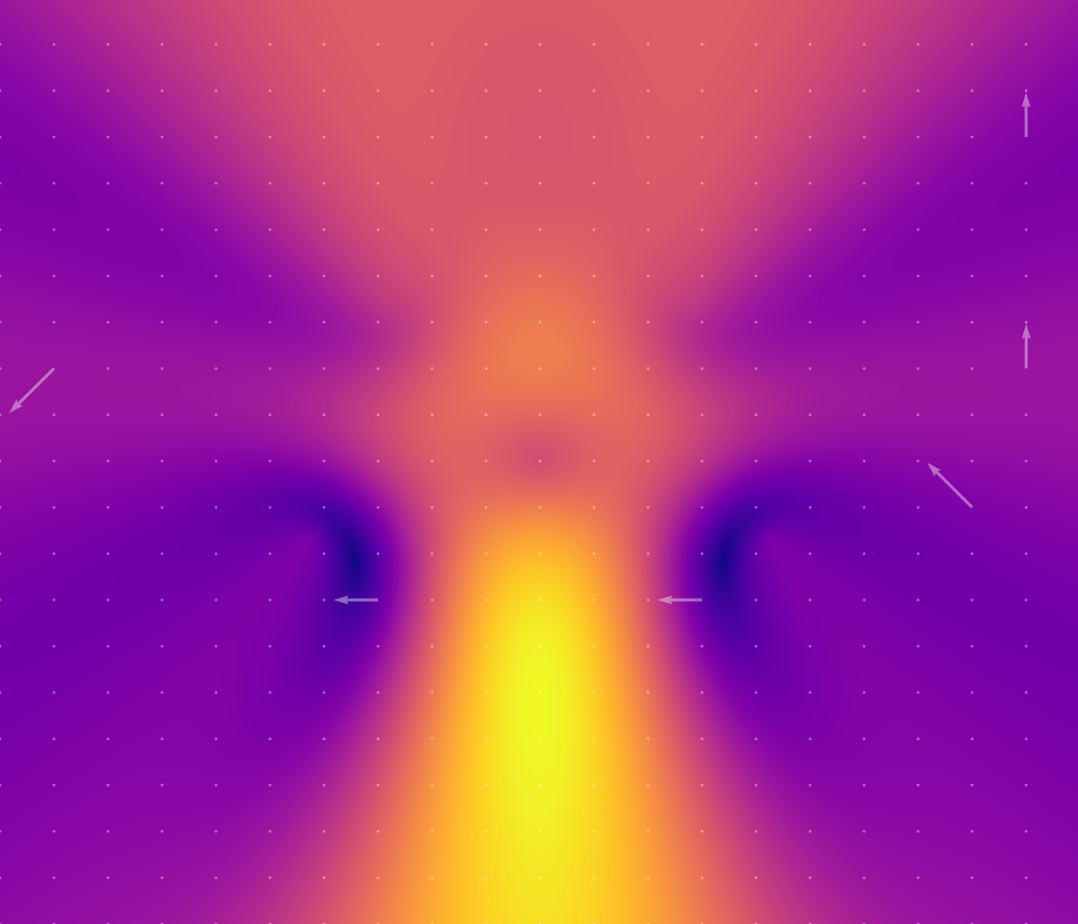
\includegraphics[width=\linewidth]{figures/tritium_modulus_vector_overlay.png}
\captionof{figure}{$\Xi$--Tritium: Five-node structure, one proton, two neutrons, two electrons.}
\end{minipage}

\vspace{1.2em}

\noindent
\begin{minipage}{0.48\textwidth}
\centering
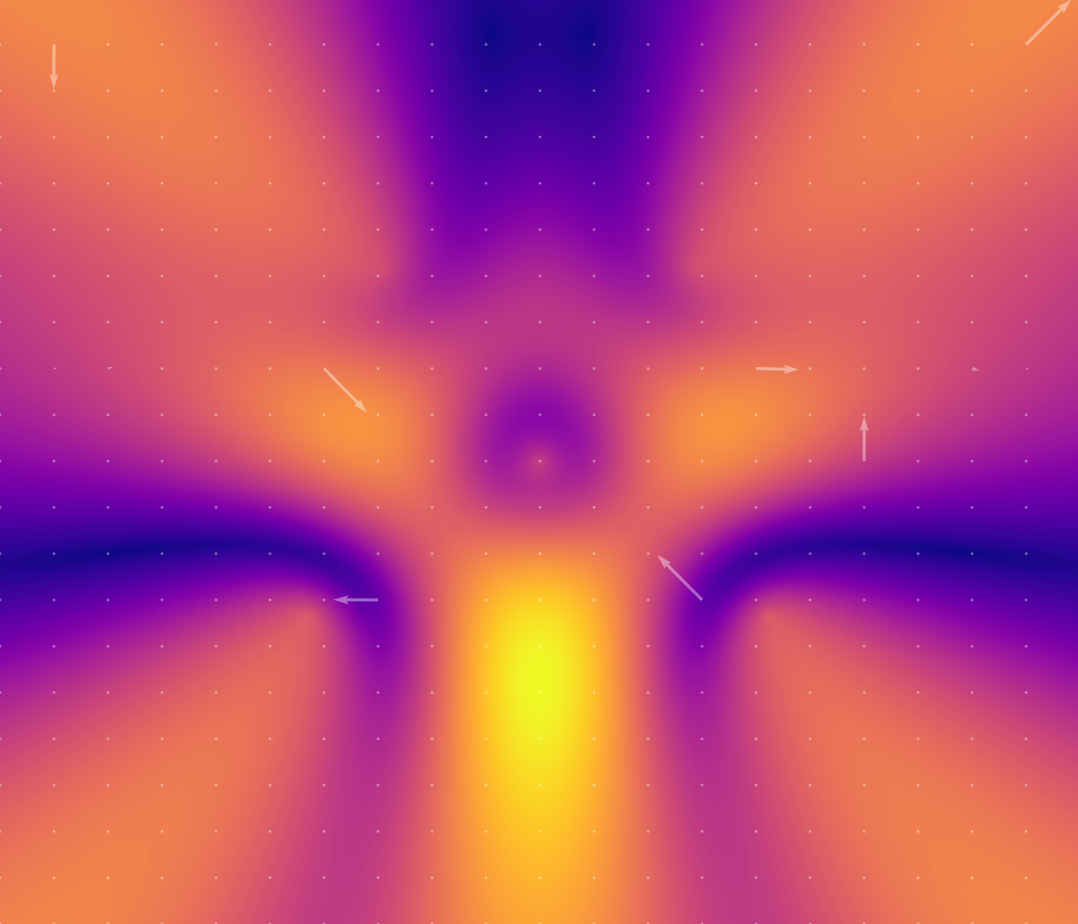
\includegraphics[width=\linewidth]{figures/water_modulus_vector_overlay.png}
\captionof{figure}{$\Xi$--Water: Central $\Xi$-oxygen phase-locked with protons, electrons.}
\end{minipage}
\hfill
\begin{minipage}{0.48\textwidth}
\centering
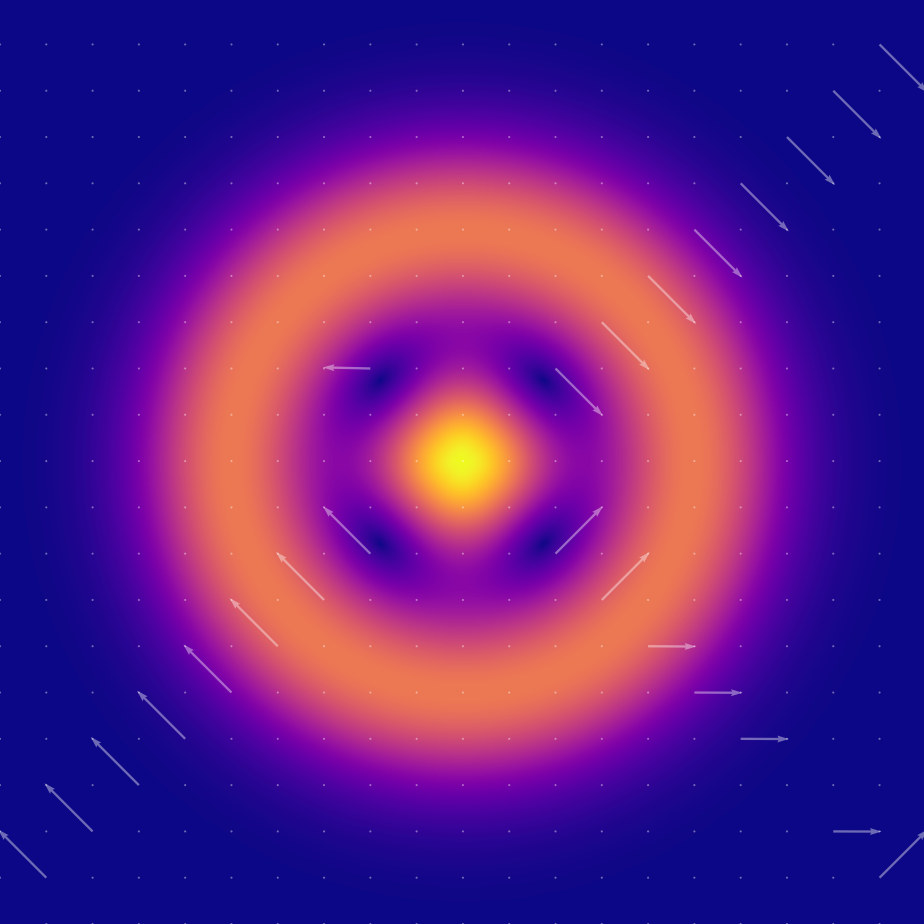
\includegraphics[width=\linewidth]{figures/xi_higgs_ignition_overlay.png}
\captionof{figure}{$\Xi$--Higgs Ignition: Phase dome at the coherence threshold.}
\end{minipage}

\vspace{1.2em}

\noindent
\begin{minipage}{0.48\textwidth}
\centering
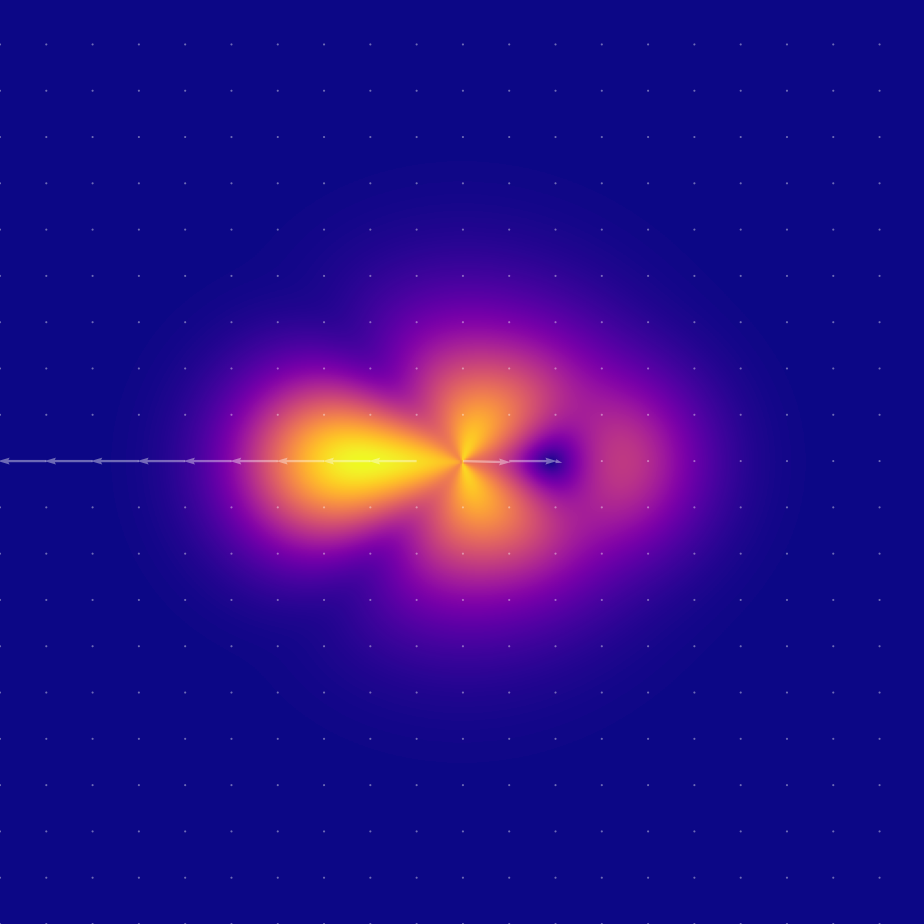
\includegraphics[width=\linewidth]{figures/xi_wz_rupture_overlay.png}
\captionof{figure}{$\Xi$--W/Z Rupture: Field shear marks topological reconfiguration.}
\end{minipage}
\hfill
\begin{minipage}{0.48\textwidth}
\centering
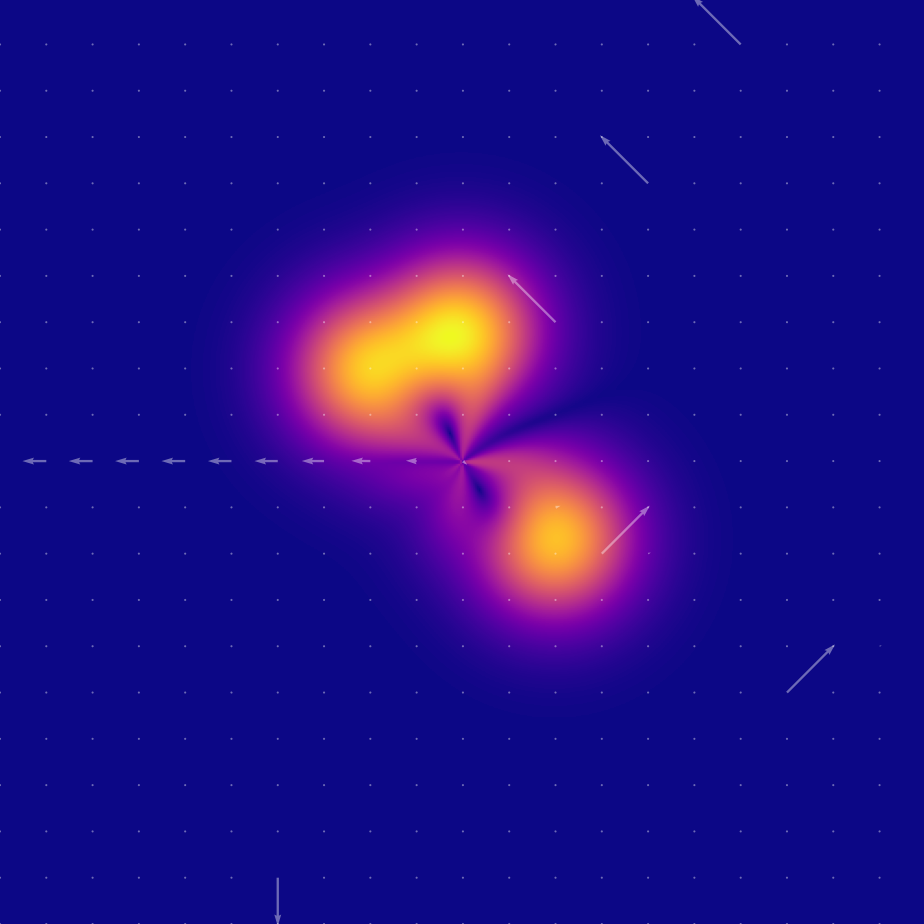
\includegraphics[width=\linewidth]{figures/xi_rho_field_overlay.png}
\captionof{figure}{$\Xi$--Rho Meson: Higher-order rebound mode, partial phase entanglement.}
\end{minipage}

\clearpage
\section*{Appendix B: GCFT Field Equations and Worked Solutions}
\addcontentsline{toc}{section}{Appendix B: GCFT Field Equations and Worked Solutions}

This appendix presents the mathematical backbone of the GCFT framework, including the full field Lagrangian, core equations of motion, analytic soliton solutions, numerical examples, and a parameter summary. All results here support the resonance structures, tables, and predictions in the main text.

\subsection*{B.1 GCFT Lagrangian and Field Equations}

The fundamental GCFT Lagrangian is:
\[
\mathcal{L} = \frac{1}{2} \partial_\mu \Xi \partial^\mu \Xi - \frac{\lambda}{4} (\Xi - \Xi_0)^4 + \beta \left(\partial_\mu \Xi \partial^\mu \Xi\right)^2
\]
where:
\begin{itemize}
  \item $\Xi$ is the complex coherence field
  \item $\lambda$ is the self-interaction coupling constant
  \item $\beta$ is the higher-order phase tension coefficient
  \item $\Xi_0$ is the vacuum field value
\end{itemize}

The Euler-Lagrange equation governing the dynamics of $\Xi$ is:
\[
\Box \Xi - \lambda (\Xi - \Xi_0)^3 + 2\beta (\partial_\nu \Xi \partial^\nu \Xi) \Box \Xi + 4\beta \partial_\mu (\partial^\mu \Xi \partial_\nu \Xi \partial^\nu \Xi) = 0
\]
where $\Box = \partial_\mu \partial^\mu$ is the d’Alembertian operator.

\subsection*{B.2 Complex Field Decomposition}

Expressing $\Xi$ in polar form,
\[
\Xi(x,t) = \rho(x,t) e^{i \theta(x,t)},
\]
where $\rho$ is the amplitude and $\theta$ is the phase, allows separation of field dynamics into amplitude modulation (mass/energy related) and phase evolution (charge/current related).

Rewriting the Lagrangian in terms of $\rho$ and $\theta$ explicitly connects coherence phase dynamics to physical observables.

\subsection*{B.3 Coherence Current and Conservation}

Define the coherence current as:
\[
J^\mu = \rho^2 \partial^\mu \theta,
\]
which satisfies the continuity equation expressing local conservation of coherence:
\[
\partial_\mu J^\mu = 0.
\]

This continuity arises naturally from the phase dynamics of $\Xi$ and is the foundation of conserved quantities such as electric charge.

\subsection*{B.4 Linearized Field Equations and Small Oscillations}

Considering small perturbations around vacuum $\Xi_0$,
\[
\Xi = \Xi_0 + \delta \Xi, \quad |\delta \Xi| \ll 1,
\]
the Euler-Lagrange equation linearizes to
\[
\Box \delta \Xi - m_\Xi^2 \delta \Xi = 0,
\]
where $m_\Xi^2 = 3 \lambda \Xi_0^2$ acts as an effective mass squared term.

This describes small oscillations akin to photon-like (massless) or massive bosonic excitations depending on field parameters, explaining why only photons propagate freely while other bosons correspond to localized rupture or ignition events.

\subsection*{B.5 Stability Analysis of Solitons}

The stability of soliton (electron) and multi-node (baryon) solutions is confirmed by evaluating the energy functional:
\[
E[\Xi] = \int \left( \frac{1}{2} |\nabla \Xi|^2 + V(\Xi) \right) d^3x,
\]
where
\[
V(\Xi) = \frac{\lambda}{4} (\Xi - \Xi_0)^4.
\]

Stable solutions minimize $E[\Xi]$, and any perturbation $\delta \Xi$ increases energy, ensuring local stability and long lifetimes of resonance structures.

\subsection*{B.6 Mass Scaling Relation}

Particle mass $m$ scales with luxion count $N$ and coherence volume $V$ as:
\[
m = \frac{N \times E_{\text{Lux}}}{V},
\]
where $E_{\text{Lux}}$ is the energy per luxion. Empirically, this is approximately 13.6 eV—the same as the ionization energy of hydrogen. In GCFT, this threshold marks the transition between stable phase-locked structures (like bound electrons) and free luxion propagation (such as ionized states).

This scale also corresponds to a characteristic decoherence time of
\[
\tau_\Xi = \frac{\hbar}{E_{\text{Lux}}} \approx \frac{6.582 \times 10^{-16}~\mathrm{eV \cdot s}}{13.6~\mathrm{eV}} \approx 48~\mathrm{as},
\]
matching the coherence loss timescales observed in ultrafast ionization dynamics. This reinforces the interpretation of luxions as coherence-carrying quanta whose compression defines mass, and whose release marks the breakdown of resonant structure.

This relation quantitatively links field coherence properties to measured particle masses—from electrons to protons and beyond—and sets the energetic ignition threshold for all GCFT field nodes.

\subsection*{B.7 Numerical Methods Overview}

Nonlinear partial differential equations governing $\Xi$ are solved using finite difference schemes with adaptive time stepping. Boundary conditions enforce $\Xi \to \Xi_0$ at spatial infinity, preserving vacuum coherence.

Convergence and stability are monitored via energy conservation and coherence measures, ensuring physically consistent numerical solutions for knots, braids, and rupture events.

\subsection*{B.8 Numerical Example: Simulated $\Xi$-Electron Knot}

\begin{figure}[H]
\centering
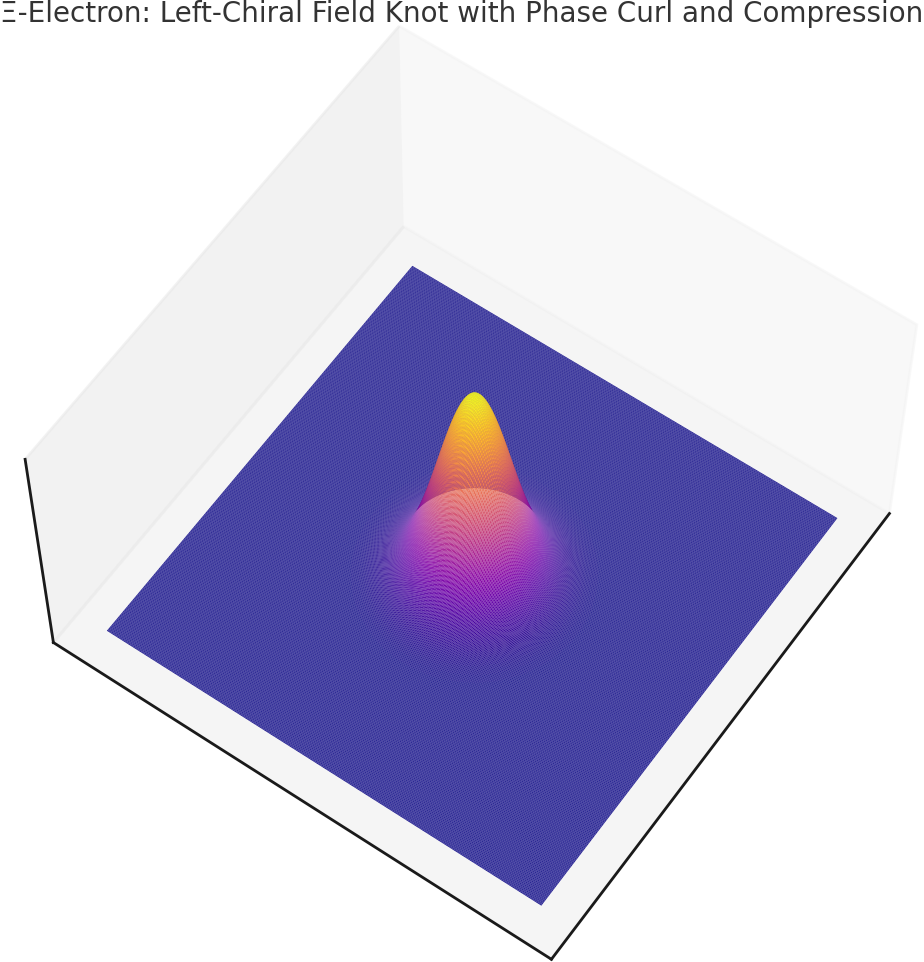
\includegraphics[width=0.5\textwidth]{figures/xi_electron_modulus_surface.png}
\caption{Numerical solution of the $\Xi$-electron: a stable knot in the field modulus matching the analytic soliton profile.}
\end{figure}

\subsection*{B.9 GCFT Decay Simulation: Neutron $\rightarrow$ Proton + $e^-$ + $\bar{\nu}_e$}

\begin{figure}[H]
\centering
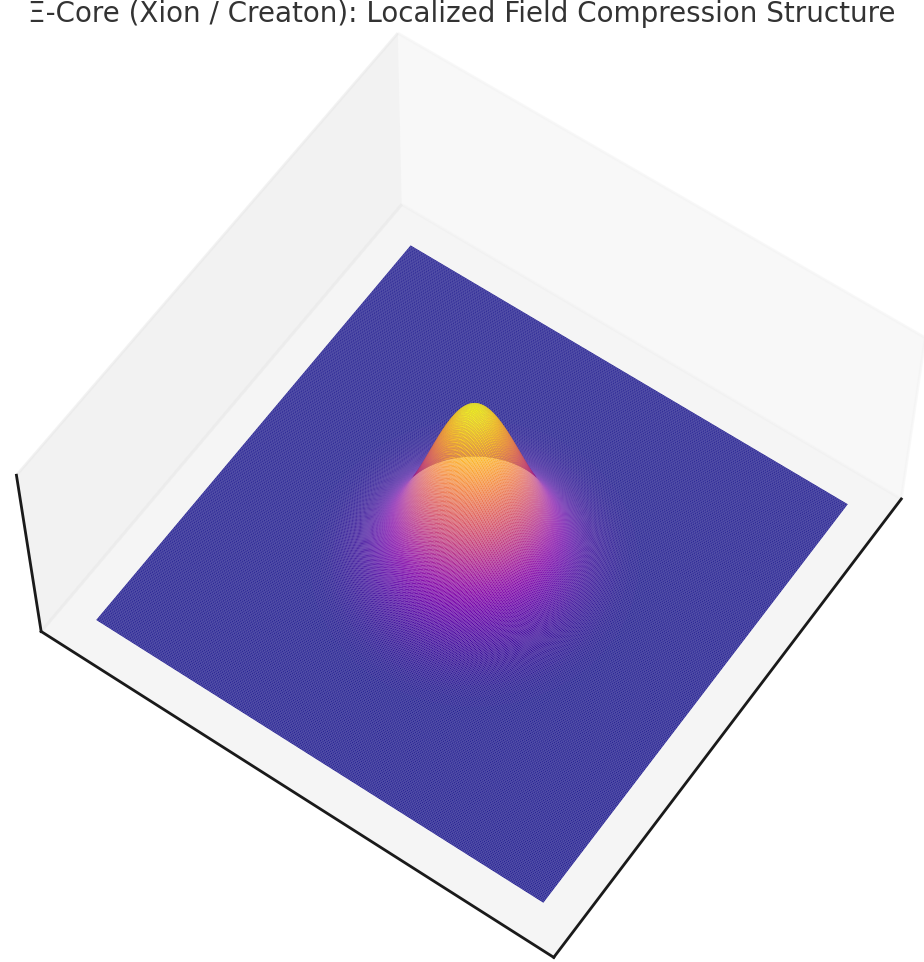
\includegraphics[width=0.5\textwidth]{figures/xi_core_modulus_surface.png}
\caption{Time evolution of $\Xi$-field during neutron decay, illustrating phase unlocking rather than force mediation.}
\end{figure}

\subsection*{B.10 Experimental Roadmap Table (Falsifiability)}

\begin{table}[H]
\small
\centering
\begin{tabular}{p{3cm} p{3cm} p{4cm} p{4cm}}
\hline
\textbf{Prediction} & \textbf{Test/Experiment} & \textbf{GCFT Signature} & \textbf{Falsification} \\
\hline
Pre-chirp in GWs & LIGO/Virgo events & Low-frequency ramp-up before merger & Absence of pre-chirp \\
Flyby anomaly & Spacecraft Doppler tracking & Clock drift, $\Delta v$ matching GCFT & No deviation from GR \\
Collider time delays & LHC, B-factories & Measurable decay timing shifts & Perfect SM decay timing \\
No free quarks & High-energy jet experiments & Only composite hadrons observed & Isolated quark detection \\
No graviton & GW detectors, tabletop tests & Absence of quantum graviton signal & Detection of graviton \\
\hline
\end{tabular}
\caption{Key GCFT predictions and their falsifiability criteria.}
\label{tab:gcft_falsification}
\end{table}



\vspace{1em}

*All field equations, solution methods, and parameter fits are referenced in the main text. For detailed derivations or code, contact the author or consult supplemental materials.*

